%%%%%%%%%%%%%%%%%%%%%%%%%%%%%%%%%%%%%%%%%
% a0poster Portrait Poster
% LaTeX Template
% Version 1.0 (22/06/13)
%
% The a0poster class was created by:
% Gerlinde Kettl and Matthias Weiser (tex@kettl.de)
% 
% This template has been downloaded from:
% http://www.LaTeXTemplates.com
%
% License:
% CC BY-NC-SA 3.0 (http://creativecommons.org/licenses/by-nc-sa/3.0/)
%
%%%%%%%%%%%%%%%%%%%%%%%%%%%%%%%%%%%%%%%%%

%----------------------------------------------------------------------------------------
%	PACKAGES AND OTHER DOCUMENT CONFIGURATIONS
%----------------------------------------------------------------------------------------

\documentclass[a0,portrait]{a0poster}

\usepackage{multicol} % This is so we can have multiple columns of text side-by-side
\columnsep=50pt % This is the amount of white space between the columns in the poster
\columnseprule=3pt % This is the thickness of the black line between the columns in the poster

\usepackage[svgnames]{xcolor} % Specify colors by their 'svgnames', for a full list of all colors available see here: http://www.latextemplates.com/svgnames-colors

\usepackage{times} % Use the times font
%\usepackage{palatino} % Uncomment to use the Palatino font

\usepackage{graphicx} % Required for including images
\graphicspath{
  {figures/},
  {figures/conformi/},
  {figures/scarti/}
}
\usepackage{booktabs} % Top and bottom rules for table
\usepackage[font=small,labelfont=bf]{caption} % Required for specifying captions to tables and figures
\usepackage{subcaption}
\usepackage{amsfonts, amsmath, amsthm, amssymb} % For math fonts, symbols and environments
\usepackage{wrapfig} % Allows wrapping text around tables and figures

\usepackage{geometry}
\geometry{paperwidth=70cm,paperheight=100cm,margin=4cm}

\usepackage[T1]{fontenc}
\usepackage[utf8]{inputenc}
\usepackage[italian]{babel}

\begin{document}

%----------------------------------------------------------------------------------------
%	POSTER HEADER 
%----------------------------------------------------------------------------------------

% The header is divided into two boxes:
% The first is 75% wide and houses the title, subtitle, names, university/organization and contact information
% The second is 25% wide and houses a logo for your university/organization or a photo of you
% The widths of these boxes can be easily edited to accommodate your content as you see fit

% SAREBBERO DA AGGIUNGERE!!!!!!!!!!!!!!!!!!!!!!!!!!!!!!!!!!!!!!!!!!!
% SAREBBERO DA AGGIUNGERE!!!!!!!!!!!!!!!!!!!!!!!!!!!!!!!!!!!!!!!!!!!
% SAREBBERO DA AGGIUNGERE!!!!!!!!!!!!!!!!!!!!!!!!!!!!!!!!!!!!!!!!!!!
%  \annoaccademico{2018-2019}
%  \corsodilaureatriennalein{Informatica}
% SAREBBERO DA AGGIUNGERE!!!!!!!!!!!!!!!!!!!!!!!!!!!!!!!!!!!!!!!!!!!
% SAREBBERO DA AGGIUNGERE!!!!!!!!!!!!!!!!!!!!!!!!!!!!!!!!!!!!!!!!!!!
% SAREBBERO DA AGGIUNGERE!!!!!!!!!!!!!!!!!!!!!!!!!!!!!!!!!!!!!!!!!!!


\begin{minipage}[cr]{0.7\linewidth}
\veryHuge \color{NavyBlue} \textbf{Autoencoder per l'Anomaly Detection applicati in ambito AutoMotive} \color{Black}\\ % Title
[.9cm]
%\begin{table}[t]
%  \begin{tabular}{ll}
%    \huge \textbf{Laureando:} & \huge \textbf{Tristano Munini}\\
%    \huge \textbf{Relatore:} & \huge \textbf{Prof. Giuseppe Serra}\\
%    \huge \textbf{Correlatore:} & \huge \textbf{Ing. Daniele Fornasier}
%  \end{tabular}
%\end{table}
\begin{tabular}{lll}
\huge \textbf{Laureando:}   && \huge \textbf{Tristano Munini}\\
\huge \textbf{Relatore:}    && \huge \textbf{Prof. Giuseppe Serra}\\
\huge \textbf{Correlatore:} && \huge \textbf{Ing. Daniele Fornasier}
\end{tabular} \\
[.5cm]

\huge Università di Udine, Dipartimento di Scienze Matematiche, Informatiche e Fisiche\\[0.1cm] % University/organization


%\Large \texttt{john@LaTeXTemplates.com} --- 1 (000) 111 1111\\
\end{minipage}
\begin{minipage}[tr]{0.3\linewidth}
  \centering
\includegraphics[width=20cm]{logo_uniud}\\
  [1cm]
  \centering
\includegraphics[width=20cm]{logo_beantech}
\end{minipage}

\vspace{1cm} % A bit of extra whitespace between the header and poster content

%----------------------------------------------------------------------------------------

\begin{multicols}{2} % This is how many columns your poster will be broken into, a portrait poster is generally split into 2 columns

%----------------------------------------------------------------------------------------
%	ABSTRACT
%----------------------------------------------------------------------------------------

\color{Navy} % Navy color for the abstract

\begin{abstract}
In questa tesi si affronta il problema di rilevare la presenza di colla sul fondo di carcasse metalliche per motori elettrici.
Il \textit{dataset} fornito, composto da qualche migliaio di immagini, comprende due classi, ma una di queste è rappresentata da un numero veramente esiguo di esemplari.
Si è deciso di utilizzare tecniche di \textit{Machine Learning} per il riconoscimento di anomalie.
In particolare è stato sviluppato un modello basato su reti neurali del tipo \textit{autoencoder}, poiché permettono di essere allenati utilizzando solamente una classe.
Applicando algoritmi di manipolazione e trasformazione delle immagini si è migliorato il \textit{dataset}.
La soluzione proposta si dimostra all'altezza dei risultati attesi, perché ha permesso di identificare quasi tutte le colle, senza però generare troppi falsi positivi.
In questo studio non è stato possibile determinare se la soluzione proposta sia applicabile in modo affidabile in ambienti industriali.
A tal fine sarebbe necessario ampliare il \textit{dataset} ed effettuare delle verifiche sul campo.
Il lavoro viene comunque considerato positivo perché ha permesso di esplorare le capacità combinate di algoritmi di manipolazione immagini e degli \textit{autoencoder}.
\end{abstract}

\color{SaddleBrown} % SaddleBrown color for the introduction
\section*{Introduzione}

%In campo industriale è sempre più frequente la scelta di integrare processi già esistenti con fotocamere per l'acquisizione di immagini.
%Le fotocamere, che hanno dimensioni sempre più ridotte ma permettono comunque di scattare fotografie ad ottima risoluzione, possono essere inserite facilmente nella maggior parte dei processi industriali, permettendo di monitorare la produzione senza comprometterla.
%Inoltre, le immagini raccolte possono andare a formare un \textit{dataset} che, utilizzato per addestrare algoritmi di \textit{machine learning}, permette non solo di monitorare il processo di produzione, ma anche di controllarlo.

I pezzi da analizzare hanno una forma cilindrica cava con una delle due estremità sigillata.
All'intero della cavità verrà alloggiato un motore elettrico per tergicristalli.
Per poter fissare il motorino è richiesto che un anello di colla sia versato sulla parete verticale interna del pezzo.
Poiché la colla è liquida è possibile che goccioli fino a raggiungere il fondo del pezzo, questo comporta il malfunzionamento del motore.
Da ciò nasce la necessità di rilevare in modo automatizzato quali pezzi presentano colla sul fondo, così da poterli scartare.
Nello specifico si vuole che il sistema riconosca il maggior numero di carcasse che presentano colla sul fondo, queste verranno poi rimosse automaticamente dal processo di produzione.
La soluzione proposta è stata sviluppata durante un tirocinio della durata di sei mesi svolto presso beanTech.
Il principale strumento utilizzato è stato il linguaggio di programmazione \textit{python}, arricchito da librerie come: \textit{opencv}, \textit{numpy}, \textit{pytorch}, \textit{matplotlib}.


\color{DarkSlateGray} % DarkSlateGray color for the rest of the content
\section*{Obiettivi}
Per quanto riguarda gli obiettivi che si vogliono raggiungere sappiamo che:
\begin{itemize}
  \item la colla viene depositata su circa $5000$ pezzi al giorno;
  \item la probabilità che gocce di colla cadano sul fondo delle carcasse è estremamente bassa.
\end{itemize}
Purtroppo non esistono dati numerici esatti ma si stima che il processo di produzione abbia un tasso d'errore di una carcassa al mese o poco più.
Questi dati possono essere trasformati in probabilità approssimative osservando che:
\begin{center}
  \begin{tabular}{ l c r }
    colla depositata al mese: & $5000 * 31 =$& $155000$ \\
    colla depositata male al mese: && $2$
  \end{tabular}
\end{center}
Quindi la probabilità che venga prodotta una carcassa non idonea è pari allo $0.00001\%$.
Il sistema di intelligenza artificiale deve riconoscere i pezzi non conformi ma soprattutto, tenendo conto della probabilità di cui sopra, deve generare un numero bassissimo di falsi positivi.
Ricordano che per falsi positivi (detti anche FP o \textit{False Positive}) si intendono tutte le carcasse che il sistema considera non conformi ma che in realtà non presentano difetti.
Un'intelligenza artificiale troppo rigida, che, quando indecisa, propende per scartare il pezzo, inciderebbe negativamente sulla produzione.
Si rischierebbe infatti di creare un enorme danno economico andando a scartare molte più carcasse del necessario.
% TODO usare teorema di bayes per dim che un modello aggressivo è peggio di uno che lascia passare
Il nostro obiettivo è creare un sistema che generi un numero di falsi positivi che sia inferiore al $2\%$, cercando di riconoscere più carcasse non conformi possibili.


\section*{Dataset}
%  \begin{center}
%    \begin{tabular}{cc} \label{griglia_fig_data}
%      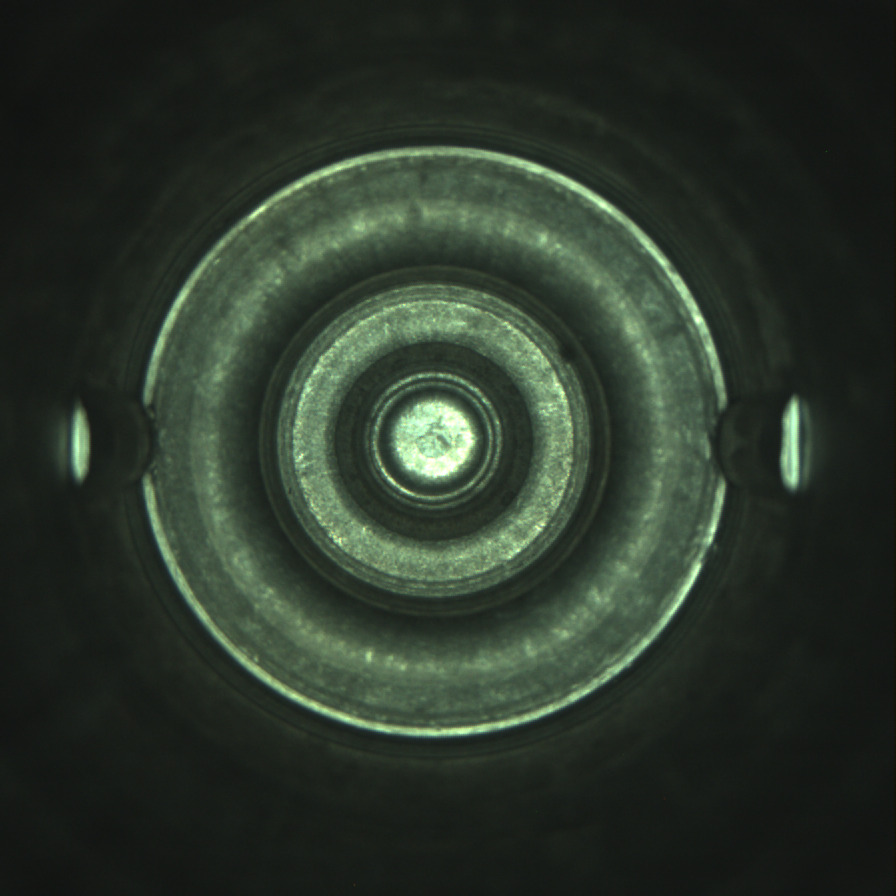
\includegraphics[width=.25\textwidth]{128___16760_0_0_1_OnLineAnalysis} &
%      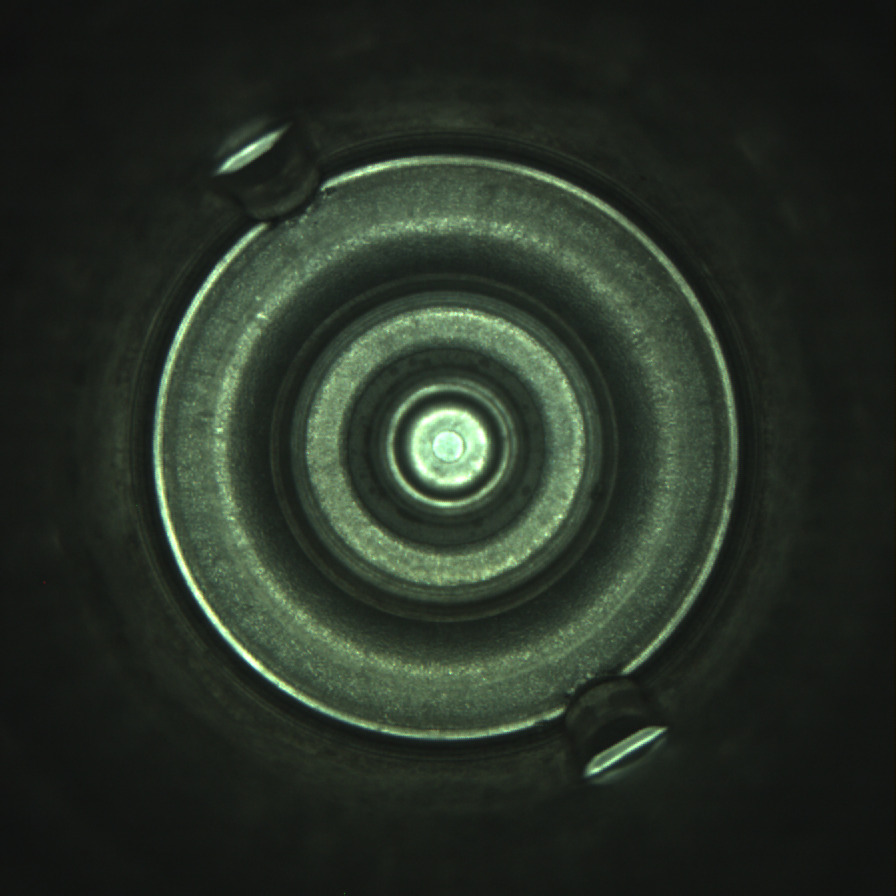
\includegraphics[width=.25\textwidth]{128___17986_1_1_1_OnLineAnalysis} \\
%      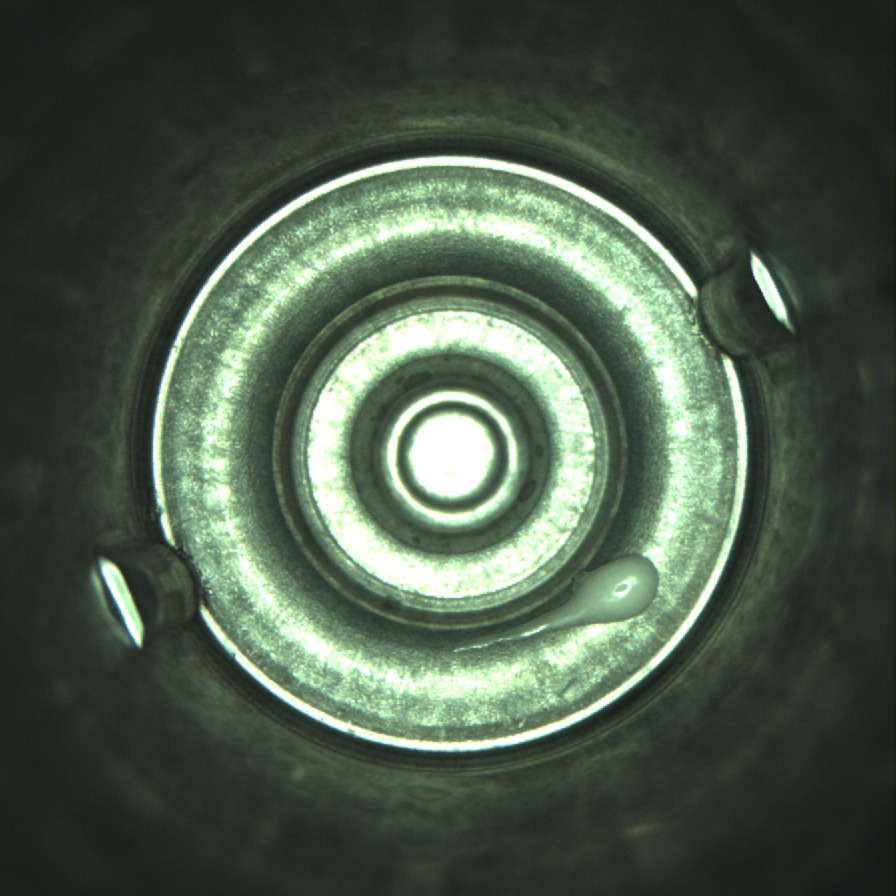
\includegraphics[width=.25\textwidth]{128___14097_1_0_1_OnLineAnalysis} &
%      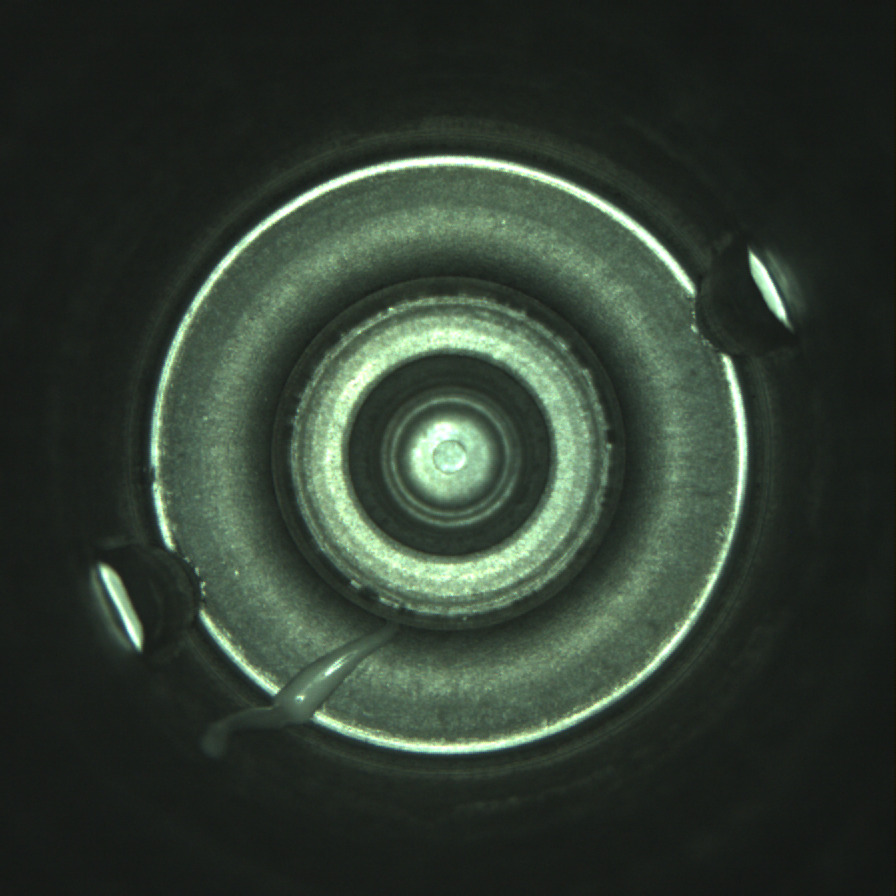
\includegraphics[width=.25\textwidth]{128___14177_1_0_1_OnLineAnalysis}
%    \end{tabular}
%    \captionof{figure}{Immagini di: ingresso, \\ uscita, differenza, risultato}
%  \end{center}
Il \textit{dataset} comprende 2000 immagini di cui solo 30 sono scarto, ovvero presentano colla sul fondo.
Da finire

\begin{center}
    \begin{tabular}{cc} \label{griglia_dataset}
      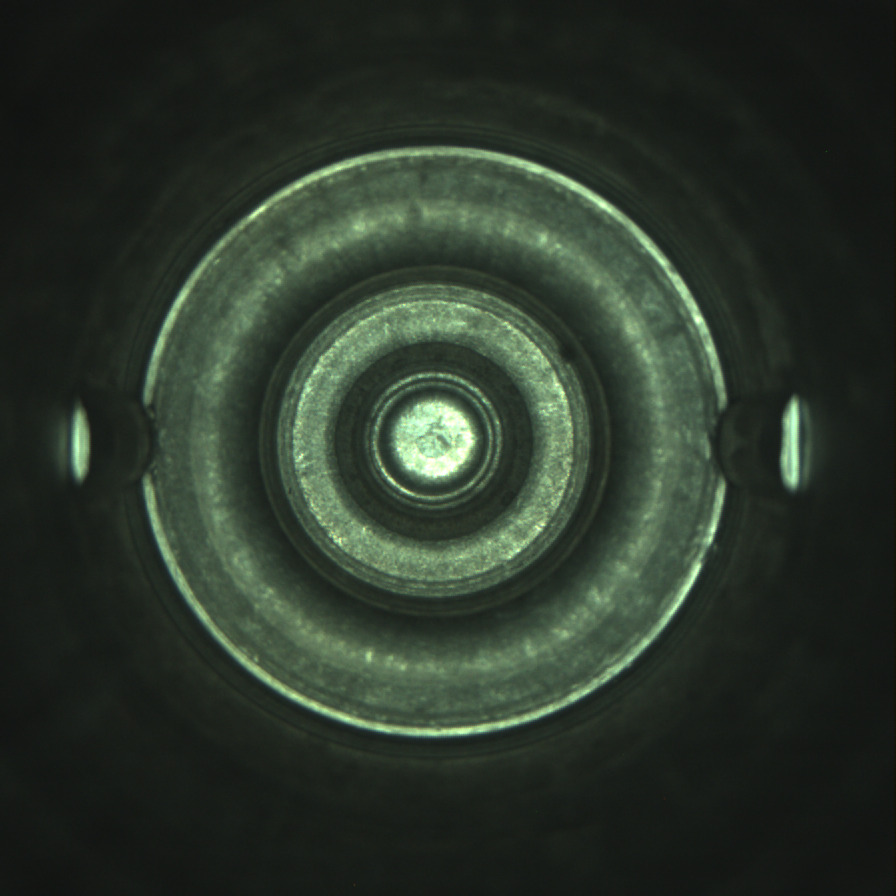
\includegraphics[width=.1\textwidth]{128___16760_0_0_1_OnLineAnalysis} &
      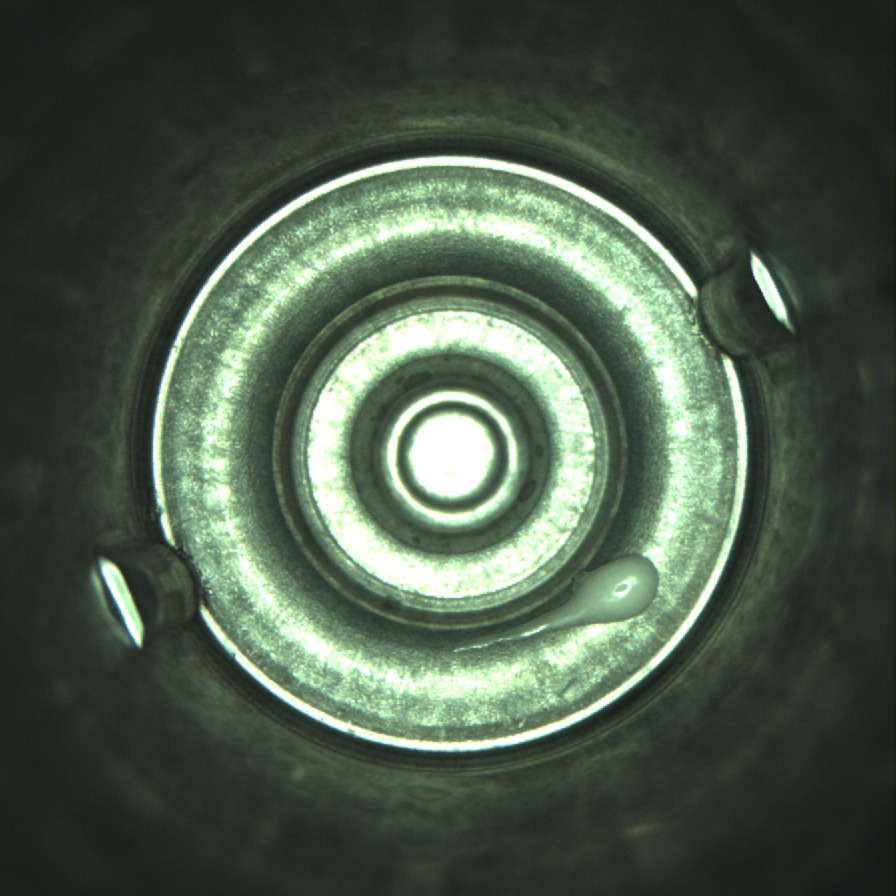
\includegraphics[width=.1\textwidth]{128___14097_1_0_1_OnLineAnalysis}
    \end{tabular}
    \captionof{figure}{Un conforme ed uno scarto}
\end{center}
  


\subsection*{Soluzione Proposta}
La soluzione proposta può essere divisa in tre momenti:
nel primo l'immagine in ingresso viene manipolata da algoritmi creati appositamente, così da ottenere un'immagine che favorisce le future trasformazioni;
l'immagine appena generata viene fornita in ingresso ad un \textit{autoencoder} con una specifica architettura;
l'\textit{output} della rete neurale viene gestito da un ulteriore algoritmo che permette di sintetizzare una classificazione binaria.

\begin{minipage}[c]{0.25\textwidth}
\centering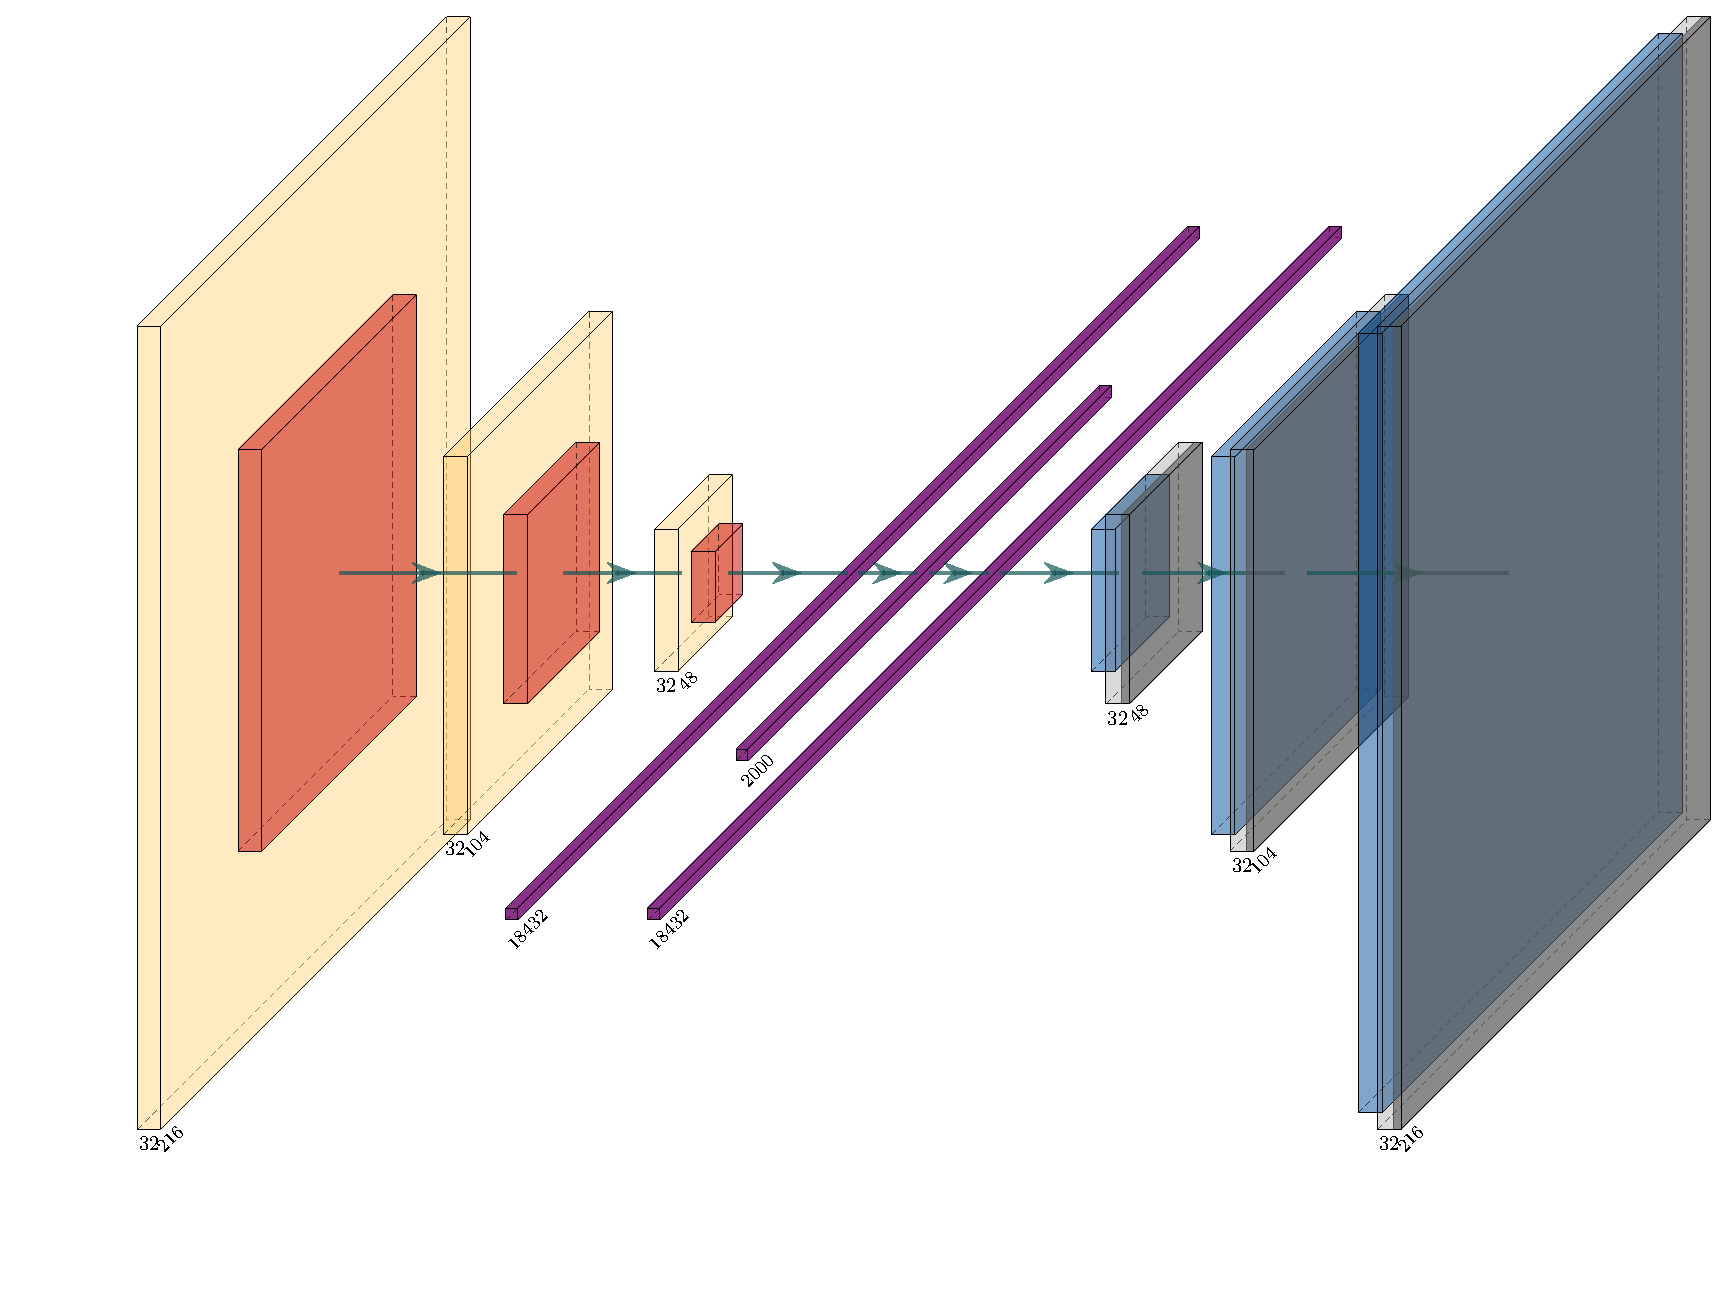
\includegraphics[width=0.9\textwidth]{ae16}
    \label{ae}
    \captionof{figure}{Architettura della rete proposta}
\end{minipage}
\begin{minipage}[c]{0.29\textwidth}
  \centering
    \begin{tabular}{cc} \label{griglia_fig}
      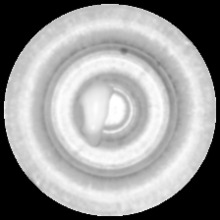
\includegraphics[width=.25\textwidth]{128___17299_0_1_1_OnLineAnalysis_con_colla_in} &
      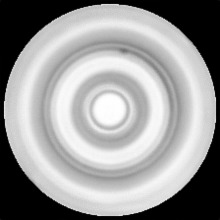
\includegraphics[width=.25\textwidth]{128___17299_0_1_1_OnLineAnalysis_con_colla_out} \\
      
\includegraphics[width=.25\textwidth]{128___17299_0_1_1_OnLineAnalysis_con_colla_to_blob} &
      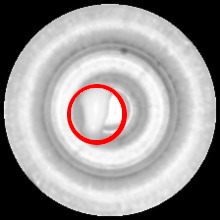
\includegraphics[width=.25\textwidth]{128___17299_0_1_1_OnLineAnalysis_con_colla_detected}
    \end{tabular}
    \captionof{figure}{Immagini di: ingresso, \\ uscita, differenza, risultato}
\end{minipage}


\section*{Risultati Ottenuti}

\begin{minipage}[c]{0.37\textwidth}
  \begin{tabular}{||l r r r||}
    \hline
    %\multicolumn{4}{||c||}{tittolo} \\ \hline
    Classe           & Elementi & Predetti come KO & Percentuale \\ \hline \hline
    Conformi         & 314      & 0                & 0\%         \\ \hline
    Scarti           & 30       & 28               & 93.3\%      \\ \hline
    Scarti sintetici & 30       & 28               & 93.3\%      \\ \hline
  \end{tabular}
\end{minipage}
\begin{minipage}[c]{0.20\textwidth}
  \begin{tabular}{||l r||}
    \hline
    Accuracy  & 0.989\% \\ \hline
    Precision & 1.000\% \\ \hline
    Recall    & 0.933\% \\ \hline
  \end{tabular}
\end{minipage}

\color{SaddleBrown} % SaddleBrown color for the conclusions to make them stand out
\section*{Conclusioni}
Osservando i risultati ottenuti si può vedere che, nonostante il campione a disposizione abbia una numerosità ridotta, nessun conforme dell'insieme di \textit{test} è stato classificato in modo scorretto.
Questo significa che c'è una quantità di falsi positivi, cioè di carcasse conformi che verrebbero scartate, pari allo 0\%.
Verificando le capacità del sistema anche sull'insieme d'allenamento, risulta che lo 1.1\% di elementi è stato classificato come scarto.
Tra questi si trovano principalmente foto scattate ad una distanza superiore alla media.
Il numero di scarti correttamente identificato corrisponde al 93.3\%.
Si può concludere che la soluzione proposta ha dato risultati vicini a quelli attesi e che quindi sia soddisfacente.
Il \textit{dataset} ristretto, però, non permette di determinare se la soluzione proposta sia applicabile in modo affidabile in ambienti industriali.
Studi futuri potrebbero comprendere un campione più ampio sia di conformi che di scarti e sperimentazioni con \textit{autoencoder} con architetture differenti.

\end{multicols}
\end{document}
